\documentclass[../../doc.tex]{subfiles}

\begin{document}

\section{Wyszukiwanie drogi}


\subsection{Stany węzłów}

\label{sec:node_states}

Rozrózniamy następujące stany węzłów:

\begin{itemize}
  \item \textit{Selected} -- pole zaklasyfikowane przez algorytm jako element końcowej ścieżki.
  \item \textit{Candidate} -- pole aktualnie analizowane przez algorytm.
  \item \textit{Queued} -- pole dodane do kolejki przetwarzania, które wkrótce stanie się polem \textit{Candidate}.
  \item \textit{Forsaken} -- pole wcześniej rozważane jako \textit{Candidate}, lecz odrzucone w dalszym przebiegu algorytmu.
\end{itemize}


Oznaczenia węzłów oraz ich stanów przedstawia \cref{fig:node_states}.

\begin{figure}[H]
  \centering
  \begin{subfigure}[b]{0.2\textwidth}
    \centering
    
\begin{tikzpicture}
      \fill[gray] (0,0) rectangle (1,1);
      \draw[black] (0,0) grid (1,1);
    \end{tikzpicture}
    \caption{Ściana.}
  \end{subfigure}%
  \hfill%
  \begin{subfigure}[b]{0.2\textwidth}
    \centering
    
\begin{tikzpicture}
      \draw[black] (0,0) grid (1,1);
    \end{tikzpicture}
    \caption{Przejście.}
  \end{subfigure}%
  \hfill%
  \begin{subfigure}[b]{0.2\textwidth}
    \centering
    \begin{tikzpicture}
      \node at (0.5, 0.5){\color{orange}\faIcon{arrows-alt}};
      \draw[black] (0,0) grid (1,1);
    \end{tikzpicture}
    \caption{Pole \textit{candidate}.}
  \end{subfigure}%
  \hfill%
  \begin{subfigure}[b]{0.2\textwidth}
    \centering
    \begin{tikzpicture}
      \draw[black] (0,0) grid (1,1);
      \node at (0.5, 0.5){\color{blue}\faIcon{home}};
    \end{tikzpicture}
    \caption{Koniec ścieżki.}
  \end{subfigure}

  \vspace{8pt}

  % \hfill%
  \begin{subfigure}[b]{0.2\textwidth}
    \centering
    \begin{tikzpicture}
      \draw[black] (0,0) grid (1,1);
      \node at (0.5, 0.5){\color{blue}\faIcon{user}};
    \end{tikzpicture}
    \caption{Pole startowe.}
  \end{subfigure}
  \hfill%
  \begin{subfigure}[b]{0.2\textwidth}
    \centering
    
\begin{tikzpicture}
      \draw[black] (0,0) grid (1,1);
      \node at (0.5, 0.5){\color{green}\faIcon{check}};
    \end{tikzpicture}
    \caption{Pole \textit{selected}.}
  \end{subfigure}
  \hfill%
  \begin{subfigure}[b]{0.2\textwidth}
    \centering
    
\begin{tikzpicture}
      \draw[black] (0,0) grid (1,1);
      \node at (0.5, 0.5){\color{red}\faIcon{skull}};
    \end{tikzpicture}
    \caption{Pole \textit{forsaken}.}
  \end{subfigure}
  \hfill%
  \begin{subfigure}[b]{0.2\textwidth}
    \centering
    
\begin{tikzpicture}
      \draw[black] (0,0) grid (1,1);
      \node at (0.5, 0.5){\color{purple}\faIcon{hourglass}};
    \end{tikzpicture}
    \caption{Pole \textit{queued}.}
  \end{subfigure}
  \caption{Oznaczenia węzłów.}
  \label{fig:node_states}
\end{figure}



\subfile{subsections/dfs/section.tex}
\subfile{subsections/bfs/section.tex}
\subfile{subsections/astar/section.tex}

\end{document}